\part{WebSocket}



\chapter{Overview}

在WebSocket出现之前,Web交互一般是基于HTTP协议的短连接或者长连接。例如,Comet\footnote{具体来说,Comet基于长轮询或iframe流来实现,仍然基于HTTP连接,其中:\newline $\bullet$ 长轮询是在打开一条连接以后保持,等待服务器推送来数据再关闭的方式。\newline $\bullet$ iframe流方式是在页面中插入一个隐藏的iframe,利用其src属性在服务器和客户端之间创建一条长链接,服务器向iframe传输数据(通常是HTML,内有负责插入信息的javascript)来实时更新页面。}曾经作为一个权宜实现来让服务器实时地将更新的信息传送到客户端,而无须客户端发出请求。



虽然WebSocket的设计初衷是用于Web浏览器和Web服务器,但是实际上可以被用于任何类型的客户端/服务器应用中。例如,WebSocket通信协议实现的是基于浏览器的原生socket,这样原先只有在C/S模式下的开发模式都可以移植到Web,从而就可以通过浏览器的支持在Web上实现与服务器端的Socket通信。


\section{Handshake}

在上述的WebSocket客户端示例中,当Web应用程序调用\textt{new WebSocket(url)}接口时,客户端就开始了与地址为url的WebServer建立握手连接的过程。


\begin{compactenum}
\item WebSocket客户端与WebSocket服务器通过TCP三次握手建立连接,如果这个建立连接失败,那么后面的过程就不会执行,WebSocket客户端将收到错误消息通知。

\item 在TCP建立连接成功后,WebSocket客户端通过http协议传送WebSocket支持的版本号、协议的子版本号、原始地址、主机地址等一些列字段给服务器端。

\item WebSocket服务器收到WebSocket客户端发送来的握手请求后,如果数据包数据和格式正确,客户端和服务器端的协议版本号匹配等,就接受本次握手连接,并给出相应的数据回复,同样回复的数据包也是采用http协议传输。

\item WebSocket客户端收到服务器回复的数据包后,如果数据包内容、格式都没有问题的话,就表示本次连接成功,触发onopen消息,此时Web开发者就可以在此时通过send接口想服务器发送数据。否则,握手连接失败,Web应用程序会收到onerror消息,并且能知道连接失败的原因。


\end{compactenum}



这个握手很像HTTP,但是实际上却不是,它允许服务器以HTTP的方式解释一部分handshake的请求,然后切换为WebSocket。


\section{Heartbeat}


心跳包就是在客户端(例如即时通信)和服务器之间定时通知对方自己状态的一个自己定义的命令字,按照一定的时间间隔定时发送,类似于心跳,所以叫做心跳包。



通常情况下,心跳包都是由客户端定时向服务器发送简单的固定信息来告诉服务器端自己还在线,并接收服务器响应的固定信息。如果服务端在规定的时间内没有收到客户端信息则将客户端视为断开。

\begin{compactitem}
\item 发包方:可以是客户端也可以是服务端,看哪边实现方便合理而定(一般是客户端)。
\item 收包方:作为收包方的服务器也可以定时轮询发心跳包,不过会消耗服务器资源。
\end{compactitem}

网络中的数据接收和发送都是使用操作系统中的Socket进行实现的,但是如果Socket已经断开,那么发送数据和接收数据的时候就一定会有问题。

\begin{compactitem}
\item 如果服务器判定客户端掉线并关闭,那么客户端后续发送的数据包被直接丢弃。
\item 如果Socket连接断开,那么服务器会继续监听客户端IP地址和端口,客户端无法将数据发送出去。
\end{compactitem}

为了判断Socket是否还可以继续使用,需要在系统中创建心跳机制,其实质就是为了保持长连接。


其实,TCP中已经为用户实现了一个叫做心跳\footnote{TCP本身实现的心跳包机制是TCP的选项,默认设置是2小时的心跳频率,不过检查不到机器断电、网线拔出、防火墙等断线类型。}的机制,如果用户设置了心跳,那么TCP就会在一定的时间(比如设置的是3秒钟)内发送当前设置的次数的心跳(比如说2次),并且此信息不会影响用户自己定义的协议。



具体来说,心跳包的内容没有什么特别规定,不过一般都是在逻辑层发送很小的包,或者只包含包头的一个空包。例如,所谓TCP“心跳”就是定时发送一个自定义的结构体(心跳包或心跳帧),可以让对方知道自己“在线”以确保连接的有效性。


如果由服务器端主动发送心跳包来检测客户端在线状态,在一定时间间隔下发送(send)一个空包给客户端后,需要客户端反馈一个同样的空包回来,那么在一定时间内收不到(recv)客户端发送过来的反馈包时,服务器就只有认定客户端掉线。

在长连接下,有可能很长一段时间都没有数据往来,而且在理论上来说,长连接是一直保持连接的,只是实际情况中中间节点出现某些故障是难以知道的。

有些情况下,有的节点(防火墙)会自动把一定时间之内没有数据交互的连接断开,因此特别需要心跳包来维持长连接的保活。

在确定客户端断线之后,服务器的逻辑逻辑层根据需求可能需要做一些事情,比如断线后的数据清理以及重新连接等,因此心跳包主要用于长连接的保活和断线处理。

一般的应用下,判定客户端断线的时间在30-40秒左右,如果对于实时性要求高,可以设置6-9秒。例如,心跳包在GRPS通信和CDMA通信的应用方面使用非常广泛,心跳包通常设定在30-40秒之间,而且数据网关会定时清理没有数据的路由。

\section{Protocol}

WebSocket是html5提出的一个协议规范,并被IETF以RFC 6455标准化,后来由W3C在Web IDL中将WebSocket API标准化。

WebSocket并不基于HTTP连接,而是在一个单独的TCP连接上提供了全双工的通信信道,而且WebSocket在TCP之上支持消息流传输,这样TCP就无需通过固定字节方式来处理流的字节数据。

或者说,WebSocket与HTTP协议一样都是基于TCP的,所以它们都是可靠的协议,用户调用的WebSocket的send函数在客户端的实现中最终都是通过TCP的系统接口进行传输的。

\begin{compactitem}
\item WebSocket服务器与WebSocket客户端之间交换的标头信息很小,大概只有2字节;
\item WebSocket客户端与WebSocket服务器都可以主动传送数据给对方;
\item 不用频繁创建TCP请求及销毁请求,减少网络带宽资源的占用,同时也节省服务器资源;
\end{compactitem}

作为一个独立的基于TCP协议的通信协议,WebSocket和HTTP的唯一关系仅仅是其握手动作被HTTP服务器解析为Upgrade请求,接下来WebSocket协议就可以在客户端和服务器之间进行更大数据量的交互,从而支持内容实时传送和实时在线游戏等。

\begin{figure}[htbp]
\centering
\includegraphics[scale=0.5]{websocket_http.png}
\caption{WebSocket协议和HTTP协议的关系}
\end{figure}

具体来说,WebSocket和HTTP协议都是应用层的协议,那么它们之间的关系是WebSocket在建立握手连接时,数据是通过HTTP协议传输的,但是在建立连接之后,真正的数据传输阶段是不需要HTTP协议参与的。

另外,在客户端和服务器基于WebSocket进行通信时,WebSocket客户端和服务器之间的通信不必在接收到客户端的请求之后才开始,这样就可以在WebSocket连接打开时直接来回传输信息,从而在客户端和服务器之间实现实时双向通信。

\begin{compactenum}
\item 打开握手


客户端与服务端建立握手,发送如下信息:

\begin{lstlisting}[language=PHP]
GET /echo HTTP/1.1
Upgrade: WebSocket
Connection: Upgrade
Host: http://www.example.org:8088
Origin: http://www.example.com
\end{lstlisting}

服务端会发回如下的响应:

\begin{lstlisting}[language=PHP]
HTTP/1.1 101 Web Socket Protocol Handshake
Upgrade: WebSocket
Connection: Upgrade
WebSocket-Origin: http://www.example.org
WebSocket-Location: ws://www.example.org:8088/echo
\end{lstlisting}

\item 数据传递
\item 关闭握手
\end{compactenum}



在浏览器和服务器之间实现的WebSocket通信可以使用标准的TCP 80端口,从而避免数据包被防火墙过滤。

\begin{figure}[htbp]
\centering
\includegraphics[scale=0.5]{websocket_process.png}
\caption{WebSocket通讯}
\end{figure}

下图显示了WebSocket通信过程的主要的三个步骤,以及在客户端和服务器端分别进行的操作。

\begin{figure}[htbp]
\centering
\includegraphics{websocket_communication.png}
\caption{WebSocket通信过程}
\end{figure}





\subsection{server}





\subsection{client}

下面的websocket客户端代码websocket.html在浏览器中运行时,使用 websocket 自动连接,发送一个消息,显示接受到的服务器响应,然后关闭连接。

WebSocket协议引入了新的URI——ws和wss来解密和加密连接,其中:

\begin{compactitem}
\item 使用ws://开头的URI表示Websocket协议;
\item 使用wss://开头的URI表示安全的WebSocket协议。
\end{compactitem}

\begin{lstlisting}[language=PHP,basicstyle=\ttfamily\footnotesize]
<!DOCTYPE html>
<html lang="en">
<head>
    <meta charset="UTF-8">
    <title>WebSocket Test</title>
    <script language="javascript" type="text/javascript">
	//申请一个WebSocket对象,参数是需要连接的服务器端的地址
        var wsUri = "ws://echo.websocket.org/";
        var output;
        function init() {
            output = document.getElementById("output");
            testWebSocket();
        }
        function testWebSocket() {
            var websocket;
            // WebSocket对象支持4个消息 onopen, onmessage, onclose和onerror
            websocket = new WebSocket(wsUri);
            // 所有的操作都是采用消息的方式触发的,
            // 这样就不会阻塞UI,使得UI有更快的响应时间。
            // 当客户端和WebSocketServer连接成功后,会触发onopen消息;
            websocket.onopen = function (evt) {
                onOpen(evt)
            };
            // 当Browser接收到WebSocketServer端发送的关闭连接请求时,就会触发onclose消息。
            websocket.onclose = function (evt) {
                onClose(evt)
            };
            // 当客户端接收到WebSocketServer发送过来的数据时,
            // 就会触发onmessage消息,参数evt中包含server传输过来的数据;
            websocket.onmessage = function (evt) {
                onMessage(evt)
            };
            // 如果连接失败,发送/接收数据失败或者处理数据出现错误,
            // 客户端会触发onerror消息
            websocket.onerror = function (evt) {
                onError(evt)
            };
        }
        function onOpen(evt) {
            writeToScreen("CONNECTED");
            doSend("WebSocket rocks");
        }
        function onClose(evt) {
            writeToScreen("DISCONNECTED");
        }
        function onMessage(evt) {
            writeToScreen('<span style="color: blue;">RESPONSE: ' + evt.data + '</span>');
            websocket.close();
        }
        function onError(evt) {
            writeToScreen('<span style="color: red;">ERROR:</span> ' + evt.data);
        }
        function doSend(message) {
            writeToScreen("SENT: " + message);
            websocket.send(message);
        }
        function writeToScreen(message) {
            var pre = document.createElement("p");
            pre.style.wordWrap = "break-word";
            pre.innerHTML = message;
            output.appendChild(pre);
        }
        window.addEventListener("load", init, false);
    </script>
</head>
<body>
<h2>WebSocket Test</h2>
<div id="output"></div>
</body>
</html>
\end{lstlisting}

客户端通过WebSocket API提供的如下4个事件进行编程:

\begin{compactitem}
\item onopen 建立连接后触发
\item onmessage 收到消息后触发
\item onerror 发生错误时触发
\item onclose 关闭连接时触发
\end{compactitem}




\begin{lstlisting}[language=PHP]

\end{lstlisting}


使用Wireshark监控到的上面WebSocket例子的数据,可以获得如下的数据:

\begin{lstlisting}[language=PHP]
GET / HTTP/1.1
Upgrade: websocket
Connection: Upgrade
Host: echo.websocket.org
Origin: null
Pragma: no-cache
Cache-Control: no-cache
Sec-WebSocket-Key: Qcgtb1RJ6HceeTRLPFux/A==
Sec-WebSocket-Version: 13
Sec-WebSocket-Extensions: x-webkit-deflate-frame
Cookie: 
__utma=9925811.951031439.1365242028.1365980711.1366068689.5; 
__utmc=9925811; 
__utmz=9925811.1365242028.1.1.utmcsr=websocket.org|utmccn=(referral)|utmcmd=referral|utmcct=/

HTTP/1.1 101 Web Socket Protocol Handshake
Upgrade: WebSocket
Connection: Upgrade
Sec-WebSocket-Accept: 84Qpane33QhxOmcz8bGkFdE1AHk=
Server: Kaazing Gateway
Date: Tue, 16 Apr 2013 09:51:25 GMT
Access-Control-Allow-Origin: null
Access-Control-Allow-Credentials: true
Access-Control-Allow-Headers: content-type
Access-Control-Allow-Headers: authorization
Access-Control-Allow-Headers: x-websocket-extensions
Access-Control-Allow-Headers: x-websocket-version
Access-Control-Allow-Headers: x-websocket-protocol
\end{lstlisting}

\begin{lstlisting}[language=PHP]

\end{lstlisting}


\section{Frame}


WebScoket协议中,数据以帧序列的形式传输。

WebSocket没有试图在HTTP之上模拟server推送,而是直接在TCP之上定义了帧协议,因此WebSocket能够支持双向的通信。

注意,所有的通信数据都是以”\textbackslash x00″开头以”\textbackslash xFF”结尾的,并且都是UTF-8编码的。

这个过程类似于HTTP的建立连接过程,不同的是在建立连接之后,接下来客户端和服务端的任何交互都需要再有这个动作。

\section{Mask}


考虑到数据安全性,客户端向服务器传输的数据帧必须进行掩码处理。服务器若接收到未经过掩码处理的数据帧,则必须主动关闭连接。

服务器向客户端传输的数据帧一定不能进行掩码处理。客户端若接收到经过掩码处理的数据帧,则必须主动关闭连接。

针对上情况,发现错误的一方可向对方发送close帧(状态码是1002,表示协议错误),以关闭连接。

\begin{figure}[htbp]
\centering
\includegraphics[scale=0.5]{websocket_close.png}
\caption{WebSocket关闭连接}
\end{figure}




\begin{lstlisting}[language=PHP]

\end{lstlisting}

\section{API}






\begin{lstlisting}[language=PHP]
enum BinaryType { "blob", "arraybuffer" };
[Constructor(DOMString url, optional (DOMString or DOMString[]) protocols), Exposed=Window,Worker]
interface WebSocket : EventTarget {
  readonly attribute DOMString url;

  // ready state
  const unsigned short CONNECTING = 0;
  const unsigned short OPEN = 1;
  const unsigned short CLOSING = 2;
  const unsigned short CLOSED = 3;
  readonly attribute unsigned short readyState;
  readonly attribute unsigned long bufferedAmount;

  // networking
           attribute EventHandler onopen;
           attribute EventHandler onerror;
           attribute EventHandler onclose;
  readonly attribute DOMString extensions;
  readonly attribute DOMString protocol;
  void close([Clamp] optional unsigned short code, optional DOMString reason);

  // messaging
           attribute EventHandler onmessage;
           attribute BinaryType binaryType;
  void send(DOMString data);
  void send(Blob data);
  void send(ArrayBuffer data);
  void send(ArrayBufferView data);
};
\end{lstlisting}





\begin{lstlisting}[language=PHP]

\end{lstlisting}




\begin{lstlisting}[language=PHP]

\end{lstlisting}



\begin{lstlisting}[language=PHP]

\end{lstlisting}



\begin{lstlisting}[language=PHP]

\end{lstlisting}




\begin{lstlisting}[language=PHP]

\end{lstlisting}




\chapter{Framework}


\section{Nodejs}

WebSocket API对于客户端而言是基于事件的,对于服务端来说可以简单的理解为实现WebSocket协议的Socket Server开发。


Nodejs可以直接使用JavaScript直接处理来自客户端的请求,这样如果服务端需要大量的业务逻辑开发,则可以直接使用node开发,因此通过node和websocket的结合可以开发出对实时性要求很高的Web应用(例如游戏、直播、股票、监控、IM等)。

NWS(Node-Websocket-Server)的原理是使用node实现websocket draft-76的协议并进行封装,同时对外提供API来方便其他应用程序调用。

NWS继承了node的http.Server的事件和方法,这样就可以简化服务端的编程,同时可以处理HTTP请求。

为了实现连接之间的通信和消息的广播,NWS实现了一个manager类来给每一个连接创建一个id,然后在内存中维护一个连接链表,并提供了上线和下线的自动管理。

NWS还提供对以下几个事件的接口,这样对于WebSocket的服务器端开发,用户已经不需要考虑WebSocket协议的实现。


\begin{compactitem}
\item listening 当服务器准备好接受客户端请求时
\item request 当一个http 请求发生时触发
\item stream
\item close
\item clientError
\item error
\end{compactitem}

NWS几乎有着和客户端浏览器上WebSocket API一样的事件,只有对连接、断开连接、消息、错误等事件进行处理,这样应用的开发就非常的灵活。

另外,node的事件驱动的机制保证了系统的高效,可以使用EventEmitter定义自己的事件触发。





下面是一个node-websocket-server提供的一个server的例子:

\begin{lstlisting}[language=PHP]
var sys = require("sys");
var ws = require('../lib/ws/server');

var server = ws.createServer({debug: true});

//handle websocket requests
server.addListener("connection",function(conn){
	conn.send("Connection: "+conn.id);
	conn.addListener("message",function(message){
		conn.broadcast("<"+conn.id+"> "+message);
		if(message == "error"){
			conn.emit("error","test");
		}
	});
});

server.addListener("error",function(){
	console.log(Array.prototype.join.call(arguments,", "));
});

server.addListener("disconnected",function(conn){
	server.broadcast("<"+conn.id+"> disconnected");
});

server.listen(8000);
\end{lstlisting}

接下来,在WebSocket客户端和服务器端打通后就可以搭建一个实时监控系统,并且直接与linux自身监控工具的结合,将监控结果通过websocket直接更到网页上。

\begin{compactitem}
\item 首先,使用node.js捕获iostat的输出

\begin{lstlisting}[language=PHP,basicstyle=\ttfamily\footnotesize]
var sys = require("sys"),
    http = require("http"),
    fs = require("fs"),
    path = require("path"),
    ws = require('../lib/ws/server');

var sys = require('sys');
var spawn = require('child_process').spawn;
var mon = spawn("iostat", ["-I", "5"]);
sys.puts("starting");
\end{lstlisting}

对于命令行输出可以使用spawn来捕获,并且在Web应用中充分利用Linux的各种系统工具。

具体来说,spawn可以根据参数启动一个进程,同时可以对stdout, stderr, exit code进行捕获。

当这些事件触发时,可以绑定我们的函数,同时捕获其输出。


\item 其次,捕获iostat的数据并发送到WebSocket客户端(这里是浏览器)

\begin{lstlisting}[language=PHP,basicstyle=\ttfamily\footnotesize]
// Handle WebSocket Requests
server.addListener("connection", function(conn) {
    conn.send("Connection: " + conn.id);
    sys.puts("Connection: " + conn.id);
    mon.stdout.on('data', function(data) {
        data = format_string(data);
        sys.puts(data);
        if (conn._state == 4)
            conn.send("#mon:" + data + "");
    });

    conn.addListener("message", function(message) {
        conn.broadcast("<" + conn.id + "> " + message);
        conn.send("<" + conn.id + "> " + message);

        if (message == "error") {
            conn.emit("error", "test");
        }
    });
});

server.addListener("error", function() {
    console.log(Array.prototype.join.call(arguments, ", "));
});

server.addListener("disconnected", function(conn) {
    server.broadcast("<" + conn.id + "> disconnected");
});

server.listen(8080);
\end{lstlisting}


\item 最后,浏览器在收到消息后,对其进行简单的字符串处理,然后就可以直接在网页中输出。

\begin{lstlisting}[language=PHP,basicstyle=\ttfamily\footnotesize]
<!DOCTYPE html>
<html>
  <head>
<title>WebSocket & Node.JS Test Page</title>
<style type="text/css">
#io_0,#io_1,#io_2 {background: blue; color: white; padding: 5px; }
#io_3,#io_4,#io_5 {background: green; color: white; padding: 5px; }
#io_6,#io_7,#io_8 {background: red; color: white; padding: 5px; }
</style>
<script src="http://ajax.googleapis.com/ajax/libs/jquery/1.4.2/jquery.min.js" type="text/javascript" charset="utf-8"></script>
</head>
<body>

<!-- KB/t tps  MB/s  us sy id   1m   5m   15m -->
<table width=480>
<thead><td colspan=3>disk</td><td colspan=3>cpu</td><td colspan=3>uptime</td></thead>
<tbody id="iotitle"></tbody>
<tbody id="iobody"></tbody>
</tr>
</table>

<form id="msgForm">
<input size=50 type="text" id="inputMessage" value="Hello" ><button
id="sendButton">Send</button>
</form>

<pre id="output"></pre>

<script>

var output = $("#output");

var log = function(s) {
    if (document.readyState !== "complete") {
        log.buffer.push(s);
    } else {
	output.prepend(s+"\n");
    }
}
log.buffer = [];
var hostname = location.hostname;
var port = location.port;
url = "ws://"+hostname+":"+port+"/echo";
w = new WebSocket(url);
w.onopen = function() {
    log("open");
    w.send("thank you for the request");
}
w.onmessage = function(e) {
	var msg = e.data;
	if(msg.match(/#mon/)) {
		var monarr = msg.split(":")[1].split(" ");
		var body = "";
		for(var item in monarr) {
			body += "<td id='io_"+item+"'>"+monarr[item]+"</td>"
		}
		$("#iobody").html(body);
		//log(monarr[0]);
		
	}
	else
    	log(e.data);
}
w.onclose = function(e) {
    log("closed");
}
function sendMessage() {
	w.send($("#inputMessage").val());
}
window.onload = function() {
	var headers = ["KB/t","tps","MB/s","user","system","idle","1m","5m","15m"];
	for(var item in headers) {
		$("#iotitle").append("<td>"+headers[item]+"</td>");
	}
    log(log.buffer.join("\n"));
    $("#msgForm").submit(function(){
    		event.preventDefault();
    		sendMessage();
    		$("#inputMessage").val("");
	})
}
</script>

</body>
</html>
\end{lstlisting}


\end{compactitem}

如果加上RGraph(基于html5),则可以打造更加精美的实时展现。

\section{Socket.IO}


Socket.IO 是一个面向实时 web 应用的 JavaScript 库,可以使服务器和客户端之间实时双向的通信成为可能。

Socket.IO有两个部分,分别是在浏览器中运行的客户端库和一个面向Node.js的服务端库,两者有着几乎一样的API,而且和Node.js一样,Socket.IO也是事件驱动的。

Socket.IO 主要使用WebSocket协议,但是如果需要的话,Socket.io可以回退到几种其它方法,例如Adobe Flash Sockets、JSONP拉取或是传统的AJAX拉取,并且在同时提供完全相同的接口。

尽管Socket.IO可以被用作WebSocket的包装库,不过它还是提供了许多其它功能,比如广播至多个套接字、存储与不同客户有关的数据和异步IO操作等。

Socket.IO 会自动选择合适的双向通信协议,仅仅需要程序员对套接字的概念有所了解,但是Socket.io并不是一个基本的、独立的、能够回退到其它实时协议的WebSocket库,它实际上是一个依赖于其它实时传输协议的自定义实时传输协议的实现。


该协议的协商部分使得支持标准WebSocket的客户端不能直接连接到Socket.io服务器,并且支持Socket.io的客户端也不能与非Socket.io框架的WebSocket或Comet服务器通信,因而Socket.io要求客户端与服务器端均须使用该框架。


\section{Swoole Framework}


PHP的Swoole扩展是一个PHP语言的高性能网络通信框架,提供了PHP语言的异步多线程服务器,异步TCP/UDP网络客户端,异步MySQL,数据库连接池,AsyncTask,消息队列,毫秒定时器,异步文件读写,异步DNS查询。

基于Swoole扩展开发的PHP Web服务器\&应用服务器内置框架,提供统一注册树、数据库操作、模板、Cache、日志、队列、上传管理和用户管理等丰富的功能特性。

与其他Web框架不同,Swoole Framework是一个全功能的后端服务器框架,因此除了Web方面的应用之外,更广泛的后端程序中都可以使用。

\begin{compactitem}
\item 内置PHP应用服务器,可脱离nginx/fpm/apache独立运行
\item 配置化与资源自动工厂,可实现从配置中创建资源对象,完全无需new对象
\item 全面采用命名空间\footnote{在彻底废弃非命名空间代码后,升级框架后需要将apps/controller/和apps/models中的代码按照命名空间的规范修改一次。}+autoload,代码中无需任何的include/require
\item 全局注册树,所有资源都挂载到全局树上,彻底实现资源的单例管理和懒加载
\item 全栈框架,提供了数据库操作,模板,Cache,日志,队列,上传管理,用户管理等几乎所有的功能
\end{compactitem}

swoole框架相比apache/fpm,主要是节省PHP框架和全局对象每次请求创建销毁带来的性能损耗。如果PHP代码是裸echo的方式,swoole框架并没有性能优势。

swoole框架给用户提供了最大的空间,与http请求无关的全局对象只需要构造一次,程序中还可以对某些对象和数据进行缓存控制。

Swoole Framework使用内置应用服务器来节省每次请求代码来的额外消耗,而且连接池技术可以很好的帮助存储系统节省连接资源。

首先,安装Swoole扩展,然后在修改php.ini或通过\texttt{dl('swoole.so')}动态载入.


\begin{lstlisting}[language=PHP]
$ cd swoole-src
$ phpize
$ ./configure
$ make && sudo make install && make clean
\end{lstlisting}

其次,下载swoole\_framework源码,放置到workspace目录中即可,其中swoole\_framework是PHP代码,只需要require/include即可,无需编译和安装。

\begin{example}
Composer
\begin{lstlisting}[language=PHP]
{
    "require": {
        "matyhtf/swoole_framework": "dev-master"
    }
}
\end{lstlisting}
\end{example}

在Swoole Framework的目录规范中,假设根目录为\texttt{\$ROOT}。

\begin{compactenum}
\item \texttt{\$ROOT/apps}

应用程序代码,此目录中的代码是公用的,包括类,配置,模板,控制器,Model等。此目录不得放置静态文件,如js, css, jpg, html等,必须全部为.php文件。此目录不允许http直接访问。

\begin{compactenum}
\item \texttt{\$ROOT/apps/controllers} Web应用的控制器类代码



\item \texttt{\$ROOT/apps/models} 数据模型封装类代码
\item \texttt{\$ROOT/apps/configs} 配置文件,通过\texttt{\$php->config['db']['master']}的形式来访问
\item \texttt{\$ROOT/apps/classes}类库,这里存放所有用户定义的类,必须符合psr-0规范,文件名必须为 \{类名\}.php,顶层命名空间必须为App。

命名空间:如 \texttt{new App\textbackslash Hello\textbackslash Test} 类会映射到 \texttt{\$ROOT/apps/classes/Hello/Test.php}

配置文件:如 \texttt{\$php->config['db']['master']}或\texttt{Swoole::getInstance()->config['db']['master']}会映射到\texttt{\$ROOT/apps/configs/db.php}文件,db.php中必须返回数组,key为master。

数据模型:\texttt{model('UserInfo')}或者\texttt{\$php->model->UserInfo}会映射到\texttt{\$ROOT/apps/models/UserInfo.php}。


\item \texttt{\$ROOT/apps/templates}模板文件目录
\end{compactenum}



\item \texttt{\$ROOT/static}

静态文件目录,比如js, css, jpg, html等。此目录允许http直接访问。

\item \texttt{\$ROOT/index.php}

web网站单一入口文件,可直接放到根目录,或者单独建立目录存放,例如\texttt{\$ROOT/webroot/index.php}

\item \texttt{\$ROOT/server.php}

服务器程序启动入口。

\end{compactenum}

swoole.ini使用ini配置文件格式,SwooleFramework会优先使用代码中指定的参数设置,其次是swoole.ini中的配置,最后是默认配置。

\subsection{App Server}


AppServer就是Swoole的内置应用服务器,需要安装Swoole Web框架的规范来写代码,所以应用程序的代码都在apps/目录中。 URL会路由到Controller的方法中,数据库的处理使用Swoole框架提供的Model或者SelectDB,模板使用smarty引擎或者直接使用php作为模板。

\begin{lstlisting}[language=PHP]
<?php
define('DEBUG', 'on');
define('WEBPATH', realpath(__DIR__ . '/../'));
require dirname(__DIR__) . '/libs/lib_config.php';

//设置PID文件的存储路径
Swoole\Network\Server::setPidFile(__DIR__ . '/app_server.pid');
/**
 * 显示Usage界面
 * php app_server.php start|stop|reload
 */
Swoole\Network\Server::start(function ()
{
    $server = Swoole\Protocol\WebServer::create(__DIR__ . '/swoole.ini');
    $server->setAppPath(WEBPATH . '/apps/');                                 //设置应用所在的目录
    $server->setDocumentRoot(WEBPATH);
    $server->setLogger(new \Swoole\Log\EchoLog(__DIR__ . "/webserver.log")); //Logger
    //$server->daemonize();                                                  //作为守护进程
    $server->run(array('worker_num' => 1, 'max_request' => 5000, 'log_file' => '/tmp/swoole.log'));
});
\end{lstlisting}


SwooleFramework应用服务器,需要安装swoole扩展,这里设置的9501就是swoole服务器监听的地址,root设置为静态文件的目录。

\begin{lstlisting}[language=PHP]
<?php
require __DIR__.'/libs/lib_config.php';

$AppServer = new Swoole\Protocol\AppServer();
$AppServer->loadSetting(__DIR__."/swoole.ini"); // 加载配置文件
$AppServer->setAppPath(__DIR__."/apps/"); // 设置应用所在的目录
$AppServer->setLogger(new Swoole\Log\EchoLog(false)); // 保存日志

/**
 *如果没有安装swoole扩展,这里还可选择
 * BlockTCP 阻塞的TCP,支持windows平台,需要将worker_num设为1
 * SelectTCP 使用select做事件循环,支持windows平台,需要将worker_num设为1
 * EventTCP 使用libevent,需要安装libevent扩展
 */

$server=new \Swoole\Network\Server('0.0.0.0',10086);
$server->setProtocol($AppServer);
$server->daemonize(); // 以守护进程形式运行
$server->run('worker_num'=>1,'max_request'=5000));
?>
\end{lstlisting}



Swoole应用服务器支持的其他特性如下:

\begin{compactitem}
\item 热部署,代码更新后即刻生效,依赖runkit扩展
\item MaxRequest进程回收机制,防止内存泄露
\item 支持使用Windows作为开发环境
\item http KeepAlive,可节省tcp connect带来的开销
\item 静态文件缓存,节省流量
\item 支持Gzip压缩,节省流量
\item 支持MySQL重新连接
\item 支持文件上传
\item 支持POST大文本
\item 支持Session/Cookie
\item 支持Http/FastCGI两种协议
\end{compactitem}

当请求静态文件是由Nginx/Apache直接处理,当请求的文件不存在时,发送给Swoole服务器来进行处理。


\begin{compactitem}

\item Nginx

\begin{example}
nginx+FPM+Swoole Framework+URL Rewrite配置
\begin{lstlisting}[language=PHP]
server {
    listen  80;
    server_name  www.swoole.com;
    root  /data/wwwroot/www.swoole.com;

    location / {
        if (!-e $request_filename){
            proxy_pass http://127.0.0.1:9501;
        }
    }
}
\end{lstlisting}
\end{example}

\item Apache

\begin{example}
Apache配置可以使用代理指令或URL Rewrite实现
\begin{lstlisting}[language=PHP]
<VirtualHost *:80>
    ServerName www.swoole.com
    DocumentRoot /data/webroot/www.swoole.com
    DirectoryIndex index.html index.php

    <Directory "/data/webroot/www.swoole.com">
        Options Indexes FollowSymLinks
            AllowOverride None
            Require all granted
    </Directory>

#   ProxyPass /admin !
#   ProxyPass /index.html !
#   ProxyPass /static !
#   ProxyPass / http://127.0.0.1:9501/

    <IfModule mod_rewrite.c>
        RewriteEngine On
        RewriteCond %{DOCUMENT_ROOT}/%{REQUEST_FILENAME} !-f
        RewriteCond %{DOCUMENT_ROOT}/%{REQUEST_FILENAME} !-d
        RewriteRule ^(.*)$ http://127.0.0.1:9501$1 [L,P]
    </IfModule>
</VirtualHost>
\end{lstlisting}
\end{example}

\end{compactitem}

在浏览器中打开http://127.0.0.1:10086/进行可以访问网站。

\subsection{Web Server}

基于php-fpm来运行swoole/framework的MVC程序,这是传统的LAMP模式,可支持静态文件和普通include php方式的程序。

Swoole Framework内置SOA逻辑层服务器/客户端,支持并行请求。

SOA这个可以很多种叫法,例如常见的RPC、远程方法调用或中间件平台等,其特点是可以跨语言、跨系统、跨网络实现业务逻辑,在后端服务方面非常重要。

swoole\_framework提供了一个高性能SOA服务器框架,并且提供了一套可并行调用服务器端的Client实现。


\begin{lstlisting}[language=PHP]
<?php
define('DEBUG', 'on');
define('WEBPATH', realpath(__DIR__ . '/../'));
require dirname(__DIR__) . '/libs/lib_config.php';


//设置PID文件的存储路径
Swoole\Network\Server::setPidFile(__DIR__ . '/app_server.pid');
/**
 * 显示Usage界面
 * php app_server.php start|stop|reload
 */
Swoole\Network\Server::start(function ()
{
    $AppSvr = new Swoole\Protocol\SOAServer;
    $AppSvr->setLogger(new \Swoole\Log\EchoLog(true)); //Logger

    /** 
     * 注册一个自定义的命名空间到SOA服务器
     * 默认使用 apps/classes
     */
    $AppSvr->addNameSpace('BL', __DIR__ . '/class');

    Swoole\Error::$echo_html = false;
    $server = Swoole\Network\Server::autoCreate('0.0.0.0', 8888);
    $server->setProtocol($AppSvr);
    //$server->daemonize(); //作为守护进程
    $server->run(
        array(
            //TODO: 实际使用中必须调大进程数
            'worker_num' => 4,
            'max_request' => 5000,
            'dispatch_mode' => 3,
            'open_length_check' => 1,
            'package_max_length' => $AppSvr->packet_maxlen,
            'package_length_type' => 'N',
            'package_body_offset' => \Swoole\Protocol\SOAServer::HEADER_SIZE,
            'package_length_offset' => 0,
        )
    );  
});
\end{lstlisting}

另外,Swoole Framework内置SMTP服务器、FtpServer和异步HttpClient。


\begin{compactitem}
\item Nginx配置

\begin{lstlisting}[language=PHP]
server {
    listen 80;
    root /home/htf/workspace/php/swoole.com;

    index           index.php index.html;
    server_name     local.swoole.com;

    location / {
        if (!-e $request_filename) {
            rewrite ^/(.*)$ /index.php;
        }
    }

    location ~ \.php$ {
        fastcgi_pass 127.0.0.1:9000;
        fastcgi_index index.php;
        include fastcgi_params;
    }
}
\end{lstlisting}

\item Apache配置

\begin{lstlisting}[language=PHP]
<VirtualHost *:80>
    ServerName www.swoole.com
    DocumentRoot /data/webroot/www.swoole.com

    <Directory "/data/webroot/www.swoole.com">
        Options Indexes FollowSymLinks
        AllowOverride None
    </Directory>

    <IfModule mod_rewrite.c>
            RewriteEngine On
            RewriteCond %{DOCUMENT_ROOT}/%{REQUEST_FILENAME} !-f
            RewriteCond %{DOCUMENT_ROOT}/%{REQUEST_FILENAME} !-d
            RewriteRule ^(.*)$ /index.php [L,P]
    </IfModule>
</VirtualHost>
\end{lstlisting}
\end{compactitem}

Swoole框架额外提供了对WebSocket网络协议的支持,并附带一个基于websocket协议的webim系统。


\subsection{Database}

修改 apps/configs/db.php ,加入配置。


\begin{compactitem}
\item charset 制定数据库字符集
\item setname 在连接服务器成功后发送\texttt{set names \$charset}
\item persistent 启用MySQL数据库长连接
\end{compactitem}


\begin{lstlisting}[language=PHP]
$db['master'] = array(
    'type'    => Swoole\Database::TYPE_MYSQLi,
    'host'    => "127.0.0.1",
    'port'    => 3306,
    'dbms'    => 'mysql',
    'engine'  => 'MyISAM',
    'user'    => "root",
    'passwd'  => "root",
    'name'    => "db_live",
    'charset' => "utf8",
    'setname' => true,
    'persistent'  => true,
);
return $db;
\end{lstlisting}

\begin{compactitem}
\item 单数据库,默认读取master配置

\begin{lstlisting}[language=PHP]
$this->db->query("select * from test");
\end{lstlisting}

\item 多数据库,读取制定的数据库配置

\begin{lstlisting}[language=PHP]
$this->db('other_db_config')->query("select * from test");
\end{lstlisting}
\end{compactitem}

swoole框架支持3种驱动类型:

\begin{compactenum}
\item Swoole\textbackslash Database::TYPE\_MYSQL,使用mysql扩展
\item Swoole\textbackslash Database::TYPE\_MYSQLi,使用mysqli扩展
\item Swoole\textbackslash Database::TYPE\_PDO,使用PDO扩展
\end{compactenum}

\texttt{Swoole\textbackslash Database->insert}将一个数组插入到数据库表中。


\begin{lstlisting}[language=PHP]
function Swoole\Database->insert(array $record, string $table_name);
$db->insert(array('field1' => 12345, 'field2' => 'hello'), 'test');
\end{lstlisting}

\begin{compactitem}
\item \texttt{\$record}是一个键值对应数组,键务必要一一对应数据库表的字段。
\item \texttt{\$table\_name}指定数据库表名。
\item 操作成功返回true,失败返回false。
\end{compactitem}

\subsection{Data ORM}


另外,可以使用\texttt{createModel('ModelName')->get(\$id)}和\texttt{createModel('ModelName')->all}来生成数据的ORM封装对象。


\begin{lstlisting}[language=PHP]
$content = $model->get(1); //这里返回的是一个Record对象
$content->title='hello world'; //Update操作
$content->save(); //保存操作,这时会执行SQL语句
echo $content->addtime; //输入值
$content->delete(); //删除此条数据

$all = $model->all();        //这里返回一个RecordSet对象
$all->filter('userid=2');    //增加一些限定条件,避免读取全部的数据库内容

//遍历符合条件的所有数据库记录
foreach($all as $obj)
{
    $obj->title = 'hello';
    echo $obj->content;
}
\end{lstlisting}


\subsection{Data Model}




数据库Model类必须继承自Swoole\textbackslash Model,必须有一个公共属性\$table来标识model对应的数据库表名。



\begin{lstlisting}[language=PHP]
class Test extends Swoole\Model
{
	public $table = 'ask_category';
}
\end{lstlisting}

另外,可选参数\$primary设置主键的字段名称,默认为\texttt{'id'}。

\begin{lstlisting}[language=PHP]
class Test extends Swoole\Model
{
	public $table = 'ask_category';
	public $primary="r_id";
}

\end{lstlisting}

\texttt{model->get}从数据库中获取单条记录:

\begin{lstlisting}[language=PHP]
function get($object_id=0,$where='')
\end{lstlisting}

参数为主键ID的值,生成的SQL类似如下:


\begin{lstlisting}[language=PHP]
SELECT * FROM table_name WHERE `id` = {$id} LIMIT 1
\end{lstlisting}

如果希望使用另外的字段进行查询,需要传入\$where参数,例如 \texttt{\$model->get('me', 'name')},则生成下面的的SQL语句,并且返回一个Record对象,在此对象上可以进行更多ORM操作。

\begin{lstlisting}[language=PHP]
SELECT * FROM table_name WHERE `name` = 'me' LIMIT 1
\end{lstlisting}

\texttt{model->set}修改单条数据库记录的内容。


\begin{lstlisting}[language=PHP]
function set($id,$data,$where='')
\end{lstlisting}

\begin{compactitem}
\item \texttt{\$id}参数为主键ID;
\item \texttt{\$where}可以指定其他字段作为查询条件。
\item \texttt{\$data}为修改的内容,必须为键值对应的数组,key将作为数据库字段名称,value为值。
\end{compactitem}


\begin{lstlisting}[language=PHP]
UPDATE table_name SET 'key' = 'value' WHERE `id` = 'id'
\end{lstlisting}

\texttt{model->del}删除单条数据库表记录。

\begin{lstlisting}[language=PHP]
function del($id,$where=null)
\end{lstlisting}


\begin{lstlisting}[language=PHP]
DELETE FROM table_name WHERE `id` = 'id'
\end{lstlisting}



\texttt{model->put}插入单条数据表记录。

\begin{lstlisting}[language=PHP]
function put($id,$where=null)
\end{lstlisting}



\begin{lstlisting}[language=PHP]
insert into table_name values(`id`,`name`) values (NULL,'value')
\end{lstlisting}

\texttt{model->gets}从数据库中获取一条记录(包含多个参数)。

\begin{lstlisting}[language=PHP]

\end{lstlisting}

\texttt{model->sets}从数据库中修改一条记录(包含多个参数)。

\begin{lstlisting}[language=PHP]

\end{lstlisting}


\texttt{model->dels}从数据库中删除一条数据(包含多个参数)。

\begin{lstlisting}[language=PHP]

\end{lstlisting}

\texttt{model->all}从数据库中获取到所有表记录。


\begin{lstlisting}[language=PHP]

\end{lstlisting}


\texttt{model->count}返回符合条件的记录数。




\begin{lstlisting}[language=PHP]

\end{lstlisting}

\texttt{model->exists}检测是否存在数据,实际可以用count代替。



\begin{lstlisting}[language=PHP]

\end{lstlisting}

\texttt{model(\$model\_name)}创建/获取Model对象,例如:

\begin{lstlisting}[language=PHP]
$object = model('UserInfo');
$object->get(10001);
\end{lstlisting}

相当于SQL语句的:

\begin{lstlisting}[language=PHP]
select * from user_info where id = 10001 limit 1
\end{lstlisting}


\texttt{table(\$table\_name)}使用数据库表名来创建一个Model,这个函数与model不同,它不需要apps/models/目录中有对应的PHP文件,直接可生成Model对象。

\begin{lstlisting}[language=PHP]
$object = table('user_info');
$object->get(10001);
\end{lstlisting}

相当于SQL语句的:


\begin{lstlisting}[language=PHP]
select * from user_info where id = 10001 limit 1
\end{lstlisting}




\subsection{Controller}




\subsection{Routing}


在\texttt{Swoole::\$php->runMVC()}调用之前可以修改默认的路由函数。


\begin{lstlisting}[language=PHP]
Swoole::$php->router(function(){
    return array('controller' => 'YourController', 'view' => 'YourView');
});
Swoole::$php->runMVC();
\end{lstlisting}

设置后将使用制定的函数作为路由,路由函数务必要返回一个数组,包含控制器和视图的名称。

\begin{lstlisting}[language=PHP]
array('controller' => 'YourController', 'view' => 'YourView');
\end{lstlisting}



\subsection{Rewrite}


swoole框架使用强规则来做URL映射,例如\texttt{http://127.0.0.1/hello/index/}将会映射到 apps/controllers/Hello.php 中的 Hello::index 方法。

用户可以修改 apps/configs/rewrite.php来增加正则配置来实现自定义URL。





\begin{lstlisting}[language=PHP]
$rewrite[] = array(
    'regx' => '^/content/([a-z]+)\.html$',
    'mvc'  => array('controller' => 'content', 'view' => 'getlist'),
    'get'  => 'app',
);
\end{lstlisting}

\begin{compactitem}
\item \texttt{\$regx}需要传入一个正则表达式,符合该正则表达式就会进入此条URL路由
\item \texttt{\$mvc}指定对应的controller, view名称
\item \texttt{\$get}可以将正则表达式中的子表达式(括号中的表达式)赋值到\$\_GET参数中
\end{compactitem}

swoole通过魔法参数提供了自动参数处理规则。

\begin{compactitem}
\item \texttt{/hello/index/100},自动赋值给 \texttt{\$\_GET['id'] = 100}
\item \texttt{/hello/index/cid-1-name-rango},自动赋值到 \texttt{\$\_GET['cid'] = 1}, \texttt{\$\_GET['name'] = 'rango'}
\end{compactitem}

\begin{lstlisting}[language=PHP]

\end{lstlisting}




\subsection{Name Space}


SwooleFramework使用了完全命名空间化的代码管理。

\begin{compactitem}
\item Swoole命名空间下的类是library类,对应目录是 \{WEBPATH\}/libs/Swoole/
\item App命名空间下是用户类,对应目录是\{WEBPATH\}/apps/classes/
\end{compactitem}


如果希望增加另外的命名空间,可以使用



\begin{lstlisting}[language=PHP]
Swoole\Loader::addNameSpace($root, $path);
\end{lstlisting}


\$root就是命名空间的根名称,\$path是对应的目录绝对路径。


\subsection{File Upload}


swoole提供了文件上传模块,可以自动处理来自HTTP POST的文件上传。

在Controller中调用下面的代码即可自动处理上传的文件。

\begin{lstlisting}[language=PHP]
$this->upload->save('Upfile_key');
//需要生成缩略图
$this->upload->thumb_width = 136; //缩略图宽度
$this->upload->thumb_height = 136; //缩略图高度
$this->upload->thumb_qulitity = 100; //缩略图质量

//自动压缩图片
$this->upload->max_width = 600; //约定图片的最大宽度
$this->upload->max_height = 600; //约定图片的最大高度
$this->upload->max_qulitity = 90; //图片压缩的质量
\end{lstlisting}


需要在apps/configs中配置upload.php,base\_dir 就是上传文件的根目录。

\begin{lstlisting}[language=PHP]
$upload = array(
    'base_dir' => WEBPATH.'/uploads/',
);
return $upload;
\end{lstlisting}


\subsection{Redis Layer}


修改 apps/configs/redis.php ,加入配置。



\begin{lstlisting}[language=PHP]
$redis['master'] = array(
    'host' => '172.19.104.157',
    'port' => 6379, //默认为6379
    //'database' => 16, //数据库ID,可选
);
\end{lstlisting}


\begin{compactitem}
\item 默认取master项作为redis配置,\texttt{\$this->redis->get},框架会读取\texttt{\$this->config['redis']['master']}作为配置
\item 使用\texttt{\$this->redis('master2')->get}实现多实例访问,框架会读取\texttt{\$this->config['redis']['master2']}作为配置
\end{compactitem}





\subsection{Socket Server}

Swoole提供了底层的网络socket服务器实现,普通用户只需要实现协议或基于现有的协议进行二次开发。

Swoole提供的底层Driver包括:

\begin{compactitem}
\item BlockTCP\footnote{BlockTCP和SelectTCP可用于Windows。}阻塞的tcp/udp server, 请求按顺序执行,必须处理完一个请求才能继续处理新的请求。
\item SelectTCP 使用select做IO复用的异步非阻塞 server,可以同时维持多个TCP连接。select最大只能维持1024个连接,并且性能会随着连接数量增多而下降
\item EventTCP 使用libevent做IO复用的异步非阻塞Server,可以同时维持大量TCP连接,性能不会随连接增多而下降
\item Server 使用Swoole扩展作为底层的网络驱动,推荐使用。
\end{compactitem}


Protocol决定应用层如何处理数据,如何回应客户端,开发者可以基于Swoole提供的Protocol之上进行开发,也可以自行实现Protocol。


Swoole Framework框架自带的Protocol有:

\begin{compactitem}
\item HttpServer 是http协议的实现,提供web server的功能
\item WebSocket 是websocket协议的实现
\item AppServer 是Web应用服务器的实现
\item SOAServer 是SOA协议的实现,(SOA不是标准协议)
\end{compactitem}

在脚本中只需要选择一种合适的Driver来构造一个Protocol对象,并调用Driver的setProtocol方法,组装到Drvier中即可,最后调用Driver的run方法进入网络事件循环即可。


\begin{example}
example.php
\begin{lstlisting}[language=PHP]
require __DIR__ . '/../libs/lib_config.php';
$AppSvr = new Swoole\Network\Protocol\HttpServer();

$AppSvr->setDocumentRoot(WEBPATH);
$AppSvr->setLogger(new \Swoole\Log\EchoLog(true)); //Logger


$server = new \Swoole\Network\SelectTCP('0.0.0.0', 8888); //这里选择了selectTCP驱动
$server->setProtocol($AppSvr); //组装协议

$server->run(array('worker_num' => 1, 'max_request' => 5000)); //运行
\end{lstlisting}
\end{example}


\begin{lstlisting}[language=PHP]
php example.php
\end{lstlisting}

\subsection{TCP Server}


\begin{compactitem}
\item Swoole\textbackslash Network\textbackslash Server 使用swoole扩展作为底层驱动
\item Swoole\textbackslash Network\textbackslash SelectTCP 使用PHP提供的stream\_select作为事件驱动方式
\item Swoole\textbackslash Network\textbackslash BlockTCP 阻塞方式的TCP
\item Swoole\textbackslash Network\textbackslash EventTCP libevent扩展作为底层驱动
\end{compactitem}

\subsection{HTTP Server}


http服务器跟fpm和apache很像,只是去包含documentRoot中的php文件,没有带有任何额外功能。 与app\_server.php不同,http\_server.php是没有携带任何Swoole Web框架功能的。



\begin{lstlisting}[language=PHP]
<?php
define('DEBUG', 'on');
define("WEBPATH", realpath(__DIR__ . '/../'));
require dirname(__DIR__) . '/libs/lib_config.php';

Swoole\Config::$debug = false;

$AppSvr = new Swoole\Protocol\HttpServer();
$AppSvr->loadSetting(__DIR__.'/swoole.ini'); //加载配置文件
$AppSvr->setDocumentRoot(__DIR__.'/webroot');
$AppSvr->setLogger(new Swoole\Log\EchoLog(true)); //Logger

Swoole\Error::$echo_html = false;

$server = Swoole\Network\Server::autoCreate('0.0.0.0', 8888);
$server->setProtocol($AppSvr);
//$server->daemonize(); //作为守护进程
$server->run(array('worker_num' => 0, 'max_request' => 5000, 'log_file' => '/tmp/swoole.log'));
\end{lstlisting}



Swoole框架提供的WebServer有3种使用方法,分别是直接使用HttpServer、继承HttpServer和使用AppServer。

\begin{compactitem}
\item 直接使用HttpServer


HttpServer支持静态文件和include file。业务代码不需要写任何Server的代码,只需要设置document\_root,并编写对应php文件。这种使用方法与Apache/Nginx+FPM类似。


\begin{example}
server.php
\begin{lstlisting}[language=PHP]
$AppSvr = new Swoole\Network\Protocol\HttpServer();
$AppSvr->loadSetting("./swoole.ini"); //加载配置文件
$AppSvr->setDocumentRoot(__DIR__.'/webdocs/'); //设置document_root

$server = new \Swoole\Network\Server('0.0.0.0', 9501);
$server->setProtocol($AppSvr);
//$server->daemonize(); //作为守护进程
$server->run(array('worker_num' => 2, 'max_request' => 1000));
\end{lstlisting}
\end{example}


\begin{example}
webdocs/index.php
\begin{lstlisting}[language=PHP]
<?php
echo "hello world";
\end{lstlisting}
\end{example}

在浏览器中打开http://localhost:9501/index.php

\item 继承HttpServer

业务代码只需要继承此类,并自行实现onRequest方法即可。

\begin{lstlisting}[language=PHP]
/**
 * 处理请求
 * @param $request
 * @return Swoole\Response
 */
function onRequest(Swoole\Request $request)
\end{lstlisting}

其中,onRequest方法参数为解析好的Request对象:

\begin{compactenum}
\item \texttt{\$request->post} : \$\_POST
\item \texttt{\$request->get} : \$\_GET
\item \texttt{\$request->cookie} : \$\_COOKIES
\item \texttt{\$request->file} : \$\_FILES
\end{compactenum}

onRequest方法必须返回一个Response对象

\begin{compactenum}
\item \texttt{\$response->body}返回的HTML内容
\item \texttt{\$response->head}HTTP头信息
\end{compactenum}

\item 使用AppServer

基于AppServer类开发,就必须遵循Swoole MVC规范, apps/目录中存放应用代码。


\begin{longtable}{|m{80pt}|m{80pt}|}
%head
\multicolumn{2}{r}{}
\tabularnewline\hline
目录	&说明
\endhead
%endhead

%firsthead
\caption{Swoole AppServer MVC规范}\\
\hline
目录	&说明
\endfirsthead
%endfirsthead

%foot
\multicolumn{2}{r}{}
\endfoot
%endfoot

%lastfoot
\endlastfoot
%endlastfoot

\hline
apps/controllers	&控制器代码\\
\hline
apps/models		&数据模型代码\\
\hline
apps/teamplets	&模板文件\\
\hline
apps/config		&配置文件\\
\hline
\end{longtable}

\end{compactitem}

\subsection{WebSocket Server}




Swoole框架提供了WebSocket协议的实现,应用程序代码只需要继承Swoole\textbackslash Network\textbackslash Protocol\textbackslash WebSocket,并实现onMessage方法即可。

onMessage方法在服务器端收到客户端消息时回调。Swoole框架已经处理好了connect/accept,打包解包等工作。应用层无需关心。

在onMessage方法中,可调用


\begin{lstlisting}[language=PHP]
$this->close($client_id) //关闭此连接
$this->send($client_id, $response_string) //向某个客户端发送数据
\end{lstlisting}

\begin{compactitem}
\item 如果你的代码中没有阻塞,建议使用Swoole扩展的SWOOLE\_BASE模式。
\item 如果业务代码中存在阻塞操作,请使用SWOOLE\_PROCESS模式,并根据实际处理时间,设置worker\_num参数,启用多进程。
\end{compactitem}


Comet是使用Http协议维持长连接来达到服务器推送的目的,而且Swoole框架提供了一套兼容WebSocket和Http 2种协议的CometServer。


\begin{compactitem}
\item 如果客户端浏览器支持WebSocket,自动使用WebSocket作为通信协议。

\item 如果客户端浏览器不支持WebSocket,则使用Comet方案。
\end{compactitem}


Comet会创建2个http请求。

\begin{compactitem}
\item /pull 此请求发出后会等待服务器推送数据。

如果在50s内未有推送信息,服务器会返回Timeout,然后客户端再次发起一次/pull/请求。
\item /push 此请求用于想服务器发送数据
\end{compactitem}

注意,pull 请求由于是启用了Http KeepAlive,实际上Socket是长连接的,不存在多次connect/close的问题,性能很高。

\begin{lstlisting}[language=PHP]

\end{lstlisting}



\begin{lstlisting}[language=PHP]

\end{lstlisting}



\begin{lstlisting}[language=PHP]

\end{lstlisting}




\begin{lstlisting}[language=PHP]

\end{lstlisting}




\begin{lstlisting}[language=PHP]

\end{lstlisting}






\chapter{swoole\_websocket\_server}


从swoole-1.7.9开始内置websocket服务器支持,swoole\_websocket\_server 继承自 swoole\_http\_server。

\begin{figure}[htbp]
\centering
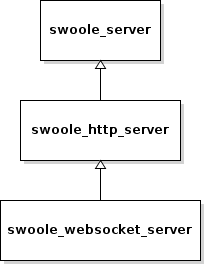
\includegraphics[scale=0.5]{swoole_server.png}
\caption{swoole\_websocket\_server的继承关系}
\end{figure}



下面的示例使用Swoole来实现一个异步非阻塞多进程的WebSocket服务器。

\begin{lstlisting}[language=PHP]
$server = new swoole_websocket_server("0.0.0.0",9501);

$server->on('open',function(swoole_websocket_server $server,$request){
	echo "server: handshake success with fd{$request->fd}\n";
});

$server->on('message',function(swoole_websocket_server $server,$frame){
	echo "receive from {$frame->fd}:{$frame->data}, opcode:{$frame->opcode},fin:{$frame->finish}\n"
	$server->push($frame->fd,"this is server");
});

$server->on('close',function($ser,$fd){
	echo "client {$d} closed\n";
});

$server->start();
\end{lstlisting}

\begin{compactitem}
\item 设置了onRequest回调,websocket服务器也可以同时作为http服务器
\item 未设置onRequest回调,websocket服务器收到http请求后会返回http 400错误页面
\end{compactitem}

\section{onHandShake}

WebSocket建立连接后进行握手,而且WebSocket服务器已经内置了handshake。

如果用户希望自己进行握手处理,可以设置onHandShake事件回调函数。





\begin{lstlisting}[language=PHP]
function onHandShake(swoole_http_request $request, swoole_http_response $response)
\end{lstlisting}

onHandShake事件回调是可选的,而且在设置onHandShake回调函数后不会再触发onOpen事件,需要应用程序代码自行处理。

\section{onOpen}

当WebSocket客户端与服务器建立连接(connect)并完成握手(handshake)后会回调onOpen函数。


\begin{lstlisting}[language=PHP]
function onOpen(swoole_websocket_server $svr,swoole_http_request $req)
\end{lstlisting}

注意,onOpen函数的第2个参数\texttt{swoole\_http\_request \$req}是从1.7.14开始的,之前是\texttt{\$fd}。

\begin{compactitem}
\item \texttt{\$req}是一个Http请求对象,包含了客户端发来的握手请求信息;
\item onOpen事件函数中可以调用push向客户端发送数据或者调用close关闭连接;
\item onOpen事件回调是可选的。
\end{compactitem}

\section{onMessage}

当服务器收到来自客户端的数据帧时会回调onMessage函数。



\begin{lstlisting}[language=PHP]
function onMessage(swoole_server $server, swoole_websocket_frame $frame)
\end{lstlisting}

\begin{compactitem}
\item \texttt{\$frame} 是swoole\_websocket\_frame对象,包含了客户端发来的数据帧信息;
\item onMessage回调必须被设置,不设置onMessage回调则服务器将无法启动。
\end{compactitem}

\subsection{swoole\_websocket\_frame}

swoole\_websocket\_frame共有4个属性,分别是:

\begin{compactitem}
\item \texttt{\$frame->fd},客户端的socket id,使用\texttt{\$server->push}推送数据时需要用到。
\item \texttt{\$frame->data},数据内容,可以是文本内容也可以是二进制数据,可以通过opcode的值来判断。
\item \texttt{\$frame->opcode},WebSocket的OpCode类型,可以参考WebSocket协议标准文档。
\item \texttt{\$frame->finish}, 表示数据帧是否完整,一个WebSocket请求可能会分成多个数据帧进行发送。
\end{compactitem}

如果\texttt{\$data}是文本类型,那么编码格式必然是UTF-8,这是WebSocket协议规定的。

\subsection{OpCode}


\begin{compactitem}
\item \texttt{WEBSOCKET\_OPCODE\_TEXT = 0x1},文本数据
\item \texttt{WEBSOCKET\_OPCODE\_BINARY = 0x2},二进制数据
\end{compactitem}

\section{push}

\texttt{swoole\_websocket\_server->push}用于向websocket客户端连接推送数据,长度最大不得超过2M。


\begin{lstlisting}[language=PHP]
function swoole_websocket_server->push(int $fd, string $data, int $opcode=1,bool $finish=true)
\end{lstlisting}

\begin{compactitem}
\item \texttt{\$fd}是客户端连接的ID,如果指定的\texttt{\$fd}对应的是TCP连接而不是websocket客户端,那么将会发送失败。
\item \texttt{\$data}是要发送的数据内容。

\item \texttt{\$opcode}用于指定发送数据内容的格式,默认为文本。

如果需要发送二进制内容,则需要设置\$opcode参数为WEBSOCKET\_OPCODE\_BINARY\_FRAME。

\item 如果发送成功返回true,发送失败则返回false。

\end{compactitem}


在实际应用中,如果Websocket服务器需要向所有连接的客户端发送广播通知消息,则可以使用foreach循环来实现。


\begin{lstlisting}[language=PHP]
foreach($server->connections as $fd){
	$server->push($fd,json_encode($data));
}
\end{lstlisting}


\subsection{Frame Type}


WebSocket数据帧类型

\begin{compactitem}
\item \texttt{WEBSOCKET\_OPCODE\_TEXT = 0x1},UTF-8文本字符数据
\item \texttt{WEBSOCKET\_OPCODE\_BINARY = 0x2},二进制数据
\end{compactitem}


\subsection{Connection State}

WebSocket连接状态

\begin{compactitem}
\item \texttt{WEBSOCKET\_STATUS\_CONNECTION = 1},连接进入等待握手
\item \texttt{WEBSOCKET\_STATUS\_HANDSHAKE = 2},正在握手
\item \texttt{WEBSOCKET\_STATUS\_FRAME = 3},已握手成功等待浏览器发送数据帧
\end{compactitem}





\begin{lstlisting}[language=PHP]

\end{lstlisting}








\begin{lstlisting}[language=PHP]

\end{lstlisting}




\begin{lstlisting}[language=PHP]

\end{lstlisting}




\begin{lstlisting}[language=PHP]

\end{lstlisting}




\begin{lstlisting}[language=PHP]

\end{lstlisting}



\begin{lstlisting}[language=PHP]

\end{lstlisting}



\begin{lstlisting}[language=PHP]

\end{lstlisting}




\begin{lstlisting}[language=PHP]

\end{lstlisting}




\begin{lstlisting}[language=PHP]

\end{lstlisting}




\begin{lstlisting}[language=PHP]

\end{lstlisting}





\begin{lstlisting}[language=PHP]

\end{lstlisting}



\begin{lstlisting}[language=PHP]

\end{lstlisting}



\begin{lstlisting}[language=PHP]

\end{lstlisting}




\begin{lstlisting}[language=PHP]

\end{lstlisting}




\begin{lstlisting}[language=PHP]

\end{lstlisting}




\begin{lstlisting}[language=PHP]

\end{lstlisting}




\begin{lstlisting}[language=PHP]

\end{lstlisting}



\begin{lstlisting}[language=PHP]

\end{lstlisting}



\begin{lstlisting}[language=PHP]

\end{lstlisting}




\begin{lstlisting}[language=PHP]

\end{lstlisting}




\begin{lstlisting}[language=PHP]

\end{lstlisting}




\begin{lstlisting}[language=PHP]

\end{lstlisting}





\begin{lstlisting}[language=PHP]

\end{lstlisting}



\begin{lstlisting}[language=PHP]

\end{lstlisting}



\begin{lstlisting}[language=PHP]

\end{lstlisting}




\begin{lstlisting}[language=PHP]

\end{lstlisting}




\begin{lstlisting}[language=PHP]

\end{lstlisting}




\begin{lstlisting}[language=PHP]

\end{lstlisting}





\begin{lstlisting}[language=PHP]

\end{lstlisting}



\begin{lstlisting}[language=PHP]

\end{lstlisting}



\begin{lstlisting}[language=PHP]

\end{lstlisting}




\begin{lstlisting}[language=PHP]

\end{lstlisting}




\begin{lstlisting}[language=PHP]

\end{lstlisting}




\begin{lstlisting}[language=PHP]

\end{lstlisting}




\begin{lstlisting}[language=PHP]

\end{lstlisting}



\begin{lstlisting}[language=PHP]

\end{lstlisting}



\begin{lstlisting}[language=PHP]

\end{lstlisting}




\begin{lstlisting}[language=PHP]

\end{lstlisting}




\begin{lstlisting}[language=PHP]

\end{lstlisting}




\begin{lstlisting}[language=PHP]

\end{lstlisting}




\begin{lstlisting}[language=PHP]

\end{lstlisting}



\begin{lstlisting}[language=PHP]

\end{lstlisting}



\begin{lstlisting}[language=PHP]

\end{lstlisting}




\begin{lstlisting}[language=PHP]

\end{lstlisting}




\begin{lstlisting}[language=PHP]

\end{lstlisting}




\begin{lstlisting}[language=PHP]

\end{lstlisting}





\begin{lstlisting}[language=PHP]

\end{lstlisting}



\begin{lstlisting}[language=PHP]

\end{lstlisting}



\begin{lstlisting}[language=PHP]

\end{lstlisting}




\begin{lstlisting}[language=PHP]

\end{lstlisting}




\begin{lstlisting}[language=PHP]

\end{lstlisting}




\begin{lstlisting}[language=PHP]

\end{lstlisting}






\begin{lstlisting}[language=PHP]

\end{lstlisting}



\begin{lstlisting}[language=PHP]

\end{lstlisting}



\begin{lstlisting}[language=PHP]

\end{lstlisting}




\begin{lstlisting}[language=PHP]

\end{lstlisting}




\begin{lstlisting}[language=PHP]

\end{lstlisting}




\begin{lstlisting}[language=PHP]

\end{lstlisting}






\begin{lstlisting}[language=PHP]

\end{lstlisting}



\begin{lstlisting}[language=PHP]

\end{lstlisting}



\begin{lstlisting}[language=PHP]

\end{lstlisting}




\begin{lstlisting}[language=PHP]

\end{lstlisting}




\begin{lstlisting}[language=PHP]

\end{lstlisting}




\begin{lstlisting}[language=PHP]

\end{lstlisting}